% Sustentación del proyecto final (12 min + 5 de preguntas). Tema UD; acento azul (logo MCIC).
% Compilar:  tectonic -Z search-path=$UD presentacion.tex   (UD = plantillas-latex del manual)
\documentclass[aspectratio=169,10pt]{beamer}
\usepackage[spanish,es-noshorthands]{babel}
\usetheme{UD}
\usepackage{booktabs}
% Generado por articulo/generar_cifras.py; no editar a mano.
\newcommand{\cifCommits}{612.811}
\newcommand{\cifDesarrollo}{558.438}
\newcommand{\cifPrueba}{54.373}
\newcommand{\cifPrevMin}{3{,}9\,\%}
\newcommand{\cifPrevMax}{4{,}5\,\%}
\newcommand{\cifPrevAnioVeintiseis}{3{,}39\,\%}
\newcommand{\cifPositivosDesarrollo}{23.735}
\newcommand{\cifPositivosPrueba}{1.947}
\newcommand{\cifCensurados}{26.133}
\newcommand{\cifAutores}{18.127}
\newcommand{\cifSubsistemas}{748}
\newcommand{\cifNVariables}{22}
\newcommand{\cifPrevQunoAdd}{0{,}9\,\%}
\newcommand{\cifPrevQcincoAdd}{11{,}7\,\%}
\newcommand{\cifReviewedIni}{0{,}42}
\newcommand{\cifReviewedFin}{0{,}71}
\newcommand{\cifFixIni}{14{,}5\,\%}
\newcommand{\cifFixFin}{18{,}4\,\%}
\newcommand{\cifValMayoritaria}{0{,}0410}
\newcommand{\cifValLogistica}{0{,}1486}
\newcommand{\cifValGB}{0{,}1578}
\newcommand{\cifParamGB}{5.645}
\newcommand{\cifParamLR}{23}
\newcommand{\cifNConfigsRef}{10}
\newcommand{\cifValFE}{0{,}1495}
\newcommand{\cifValFEde}{0{,}0053}
\newcommand{\cifValVariante}{0{,}1206}
\newcommand{\cifReglasMin}{3}
\newcommand{\cifReglasMax}{6}
\newcommand{\cifAntMin}{3}
\newcommand{\cifAntMax}{10}
\newcommand{\cifTiempoFE}{11}
\newcommand{\cifNBusqueda}{14}
\newcommand{\cifMejorBusqueda}{0{,}1485}
\newcommand{\cifRazonValFE}{94{,}8\,\%}
\newcommand{\cifCongelada}{2026-11-07 23:41}
\newcommand{\cifHuella}{11e7039f3cc27912}
\newcommand{\cifSemillaRef}{11}
\newcommand{\cifSensMax}{0{,}1498}
\newcommand{\cifSensMaxR}{10}
\newcommand{\cifSensMaxPm}{0{,}05}
\newcommand{\cifSensMin}{0{,}1305}
\newcommand{\cifSensMinR}{15}
\newcommand{\cifSensMinPm}{0{,}30}
\newcommand{\cifSensMutBaja}{0{,}1486}
\newcommand{\cifSensMutAlta}{0{,}1347}
\newcommand{\cifReglasVariante}{15}
\newcommand{\cifAntVariante}{29}
\newcommand{\cifRegReferencias}{30}
\newcommand{\cifRegPropuesto}{84}
\newcommand{\cifRegBusq}{42}
\newcommand{\cifRegSens}{24}
\newcommand{\cifTestMay}{0{,}0346}
\newcommand{\cifTestMayde}{0{,}0000}
\newcommand{\cifTestMayic}{[0{,}033;\ 0{,}036]}
\newcommand{\cifCaidaMay}{15{,}5\,\%}
\newcommand{\cifTestLR}{0{,}1274}
\newcommand{\cifTestLRde}{0{,}0000}
\newcommand{\cifTestLRic}{[0{,}117;\ 0{,}140]}
\newcommand{\cifCaidaLR}{14{,}2\,\%}
\newcommand{\cifTestGB}{0{,}1320}
\newcommand{\cifTestGBde}{0{,}0007}
\newcommand{\cifTestGBic}{[0{,}121;\ 0{,}146]}
\newcommand{\cifCaidaGB}{16{,}3\,\%}
\newcommand{\cifTestVar}{0{,}0901}
\newcommand{\cifTestVarde}{0{,}0000}
\newcommand{\cifTestVaric}{[0{,}083;\ 0{,}098]}
\newcommand{\cifCaidaVar}{25{,}3\,\%}
\newcommand{\cifTestFE}{0{,}1202}
\newcommand{\cifTestFEde}{0{,}0024}
\newcommand{\cifTestFEic}{[0{,}108;\ 0{,}128]}
\newcommand{\cifCaidaFE}{19{,}5\,\%}
\newcommand{\cifPrevPrueba}{3{,}46\,\%}
\newcommand{\cifNPrueba}{54.373}
\newcommand{\cifCuno}{91{,}1\,\%}
\newcommand{\cifFriedmanP}{0{,}0043}
\newcommand{\cifNemenyiCD}{3{,}05}
\newcommand{\cifAssistedN}{2.031}
\newcommand{\cifAssistedPrev}{2{,}81\,\%}
\newcommand{\cifAssistedLR}{0{,}079}
\newcommand{\cifSinAssistedLR}{0{,}130}
\newcommand{\cifAssistedGB}{0{,}067}
\newcommand{\cifSinAssistedGB}{0{,}136}
\newcommand{\cifAssistedFE}{0{,}055}
\newcommand{\cifSinAssistedFE}{0{,}120}
\newcommand{\cifFEMarcMin}{0{,}0\,\%}
\newcommand{\cifFEMarcMax}{17{,}9\,\%}
\newcommand{\cifFEMccMin}{0{,}000}
\newcommand{\cifFEMccMax}{0{,}175}
\newcommand{\cifFEApMin}{0{,}1172}
\newcommand{\cifFEApMax}{0{,}1245}
\newcommand{\cifFERefMarc}{17{,}9\,\%}
\newcommand{\cifFERefAp}{0{,}1172}
\newcommand{\cifMcAciertaGB}{584}
\newcommand{\cifMcFallaGB}{4.379}
\newcommand{\cifMcAciertaLR}{667}
\newcommand{\cifMcFallaLR}{3.422}
\newcommand{\cifMcAciertaVar}{3.306}
\newcommand{\cifMcFallaVar}{878}
\newcommand{\cifNReglasRef}{5}
\newcommand{\cifParamFE}{27}
\newcommand{\cifParamGBprueba}{5.765}
\newcommand{\cifErrQcincoSens}{86{,}8\,\%}
\newcommand{\cifErrQcincoPrev}{9{,}6\,\%}
\newcommand{\cifErrQunoPrev}{0{,}8\,\%}
\newcommand{\cifErrFixAp}{0{,}088}
\newcommand{\cifErrNoFixAp}{0{,}126}
\newcommand{\cifErrFixSens}{20{,}3\,\%}
\newcommand{\cifErrNoFixSens}{58{,}7\,\%}
\newcommand{\cifMesIni}{0{,}151}
\newcommand{\cifMesFin}{0{,}086}
\newcommand{\cifMesGBIni}{0{,}158}
\newcommand{\cifMesGBFin}{0{,}104}
\newcommand{\cifRangoFE}{2{,}50}
\newcommand{\cifRangoGB}{1{,}00}
\newcommand{\cifRangoLR}{2{,}50}
\newcommand{\cifRangoVar}{4{,}00}
\newcommand{\cifRangoMay}{5{,}00}
\newcommand{\cifAporteEvolPrueba}{33\,\%}
\newcommand{\cifItDosCreOriFE}{0{,}1485}
\newcommand{\cifItDosCreOriGB}{0{,}1578}
\newcommand{\cifItDosCreOriRazon}{0{,}941}
\newcommand{\cifItDosCreAmpFE}{0{,}1472}
\newcommand{\cifItDosCreAmpGB}{0{,}1578}
\newcommand{\cifItDosCreAmpRazon}{0{,}933}
\newcommand{\cifItDosDesOriFE}{0{,}1478}
\newcommand{\cifItDosDesOriGB}{0{,}1577}
\newcommand{\cifItDosDesOriRazon}{0{,}937}
\newcommand{\cifItDosDesAmpFE}{0{,}1428}
\newcommand{\cifItDosDesAmpGB}{0{,}1577}
\newcommand{\cifItDosDesAmpRazon}{0{,}905}
\newcommand{\cifItDosUmbral}{0{,}947}
\newcommand{\cifItDosAdoptada}{no}

% Generado por revision/generar_e1.py; no editar a mano.
\newcommand{\nArxivQuno}{35}
\newcommand{\nArxivQdos}{3}
\newcommand{\nArxivTotal}{38}
\newcommand{\nArxivDup}{0}
\newcommand{\nOaQuno}{162}
\newcommand{\nOaQdos}{33}
\newcommand{\nOaTotal}{195}
\newcommand{\nOaDup}{39}
\newcommand{\nDup}{39}
\newcommand{\nTamizados}{194}
\newcommand{\nExclTitulo}{147}
\newcommand{\nPasan}{47}
\newcommand{\nExclTexto}{10}
\newcommand{\nIncluidosBases}{37}
\newcommand{\nOtros}{21}
\newcommand{\nTotalIncluidos}{58}
\newcommand{\nMatriz}{16}
\newcommand{\nMatrizRecientes}{13}
\newcommand{\nRecientes}{49}
\newcommand{\nTextoCompleto}{35}
\newcommand{\nSoloResumen}{23}
\newcommand{\fechaConsulta}{2026-11-06}
\newcommand{\fechaConsultaOa}{2026-11-07}

\newcommand{\dato}[2]{{\fontsize{17pt}{19pt}\selectfont\bfseries\color{UDBlue}#1}\\[1pt]{\fontsize{7.5pt}{8.5pt}\selectfont #2}}

\begin{document}

\UDportada{¿Sobrevive un clasificador\\difuso-evolutivo a 2026?}
          {Riesgo de commits del kernel de Linux}
          {Juan Felipe Rodríguez Galindo\\{\fontsize{6.4pt}{7.4pt}\selectfont\mdseries\color{UDSilver}20261595004}}
          {Maestría en Ciencias de la Información y las Comunicaciones}
          {Inteligencia Computacional, 2026}

%-------------------------------------------------------------------
\begin{frame}{El problema}{Qué commits van a necesitar una corrección}
  \begin{columns}[T,onlytextwidth]
    \begin{column}{0.56\textwidth}
      \UDCard{white}{UDBorder}{\cardtitle{UDBlue}{Etiqueta explícita}{\fontsize{8.5pt}{10.5pt}\selectfont
      En el kernel, el trailer \texttt{Fixes:} de un commit posterior señala al culpable. Un commit es \textbf{riesgoso} si alguien lo cita así en $\le$ 90 días.}}
      \vspace{0.18cm}
      \UDCard{white}{UDBorder}{\cardtitle{UDBlue}{2026: llega la IA}{\fontsize{8.5pt}{10.5pt}\selectfont
      v7.0 pide declarar \texttt{Assisted-by:}; en octubre se retira porque solo $\sim$10\,\% lo declaraba. La era IA se define por fecha.}}
    \end{column}
    \begin{column}{0.40\textwidth}
      \UDCard{UDLightGray}{UDBlue!60}{\cardtitle{UDBlue}{Pregunta}{\fontsize{8.5pt}{10.5pt}\selectfont
      ¿Un clasificador de $\le$15 reglas difusas ajustadas con un algoritmo genético \textbf{mantiene} su desempeño de 2019--2025 en 2026?}}
      \vspace{0.18cm}
      {\fontsize{8pt}{9.5pt}\selectfont\textbf{Éxito} (fijado antes):\\
      C1 AUC-PR $\ge$ 90\,\% del mejor clásico\\
      C2 cae menos que ese clásico\\
      C3 IC excluye la prevalencia + McNemar}
    \end{column}
  \end{columns}
  \note{2 min. Problema y por qué 2026 es interesante.}
\end{frame}

%-------------------------------------------------------------------
\begin{frame}{Estado del arte y brecha}{\nTotalIncluidos{} trabajos verificados en arXiv y OpenAlex (PRISMA)}
  \begin{columns}[T,onlytextwidth]
    \begin{column}{0.48\textwidth}
      {\fontsize{8.5pt}{10.5pt}\selectfont
      \begin{itemize}
        \item JIT se valida casi siempre con un corte o validación cruzada, y se mide con AUC-ROC o F1.
        \item A nivel de commit, lo difuso y lo evolutivo solo son piezas auxiliares (ponderar, agrupar, ajustar).
        \item La deriva está demostrada, pero ningún estudio reporta AUC-PR.
        \item En el kernel, con la prevalencia real, el PR-AUC cae de 0,805 a 0,016.
      \end{itemize}}
    \end{column}
    \begin{column}{0.48\textwidth}
      \UDCard{UDLightGray}{UDBlue!60}{\cardtitle{UDBlue}{Brecha}{\fontsize{8.5pt}{10.5pt}\selectfont
      No hay un clasificador de reglas difusas evolucionado a nivel de commit, evaluado con partición temporal y AUC-PR, ni medido en 2026.}}
    \end{column}
  \end{columns}
\end{frame}

%-------------------------------------------------------------------
\begin{frame}{Datos}{Minería del historial completo de \texttt{torvalds/linux}}
  \begin{columns}[T,onlytextwidth]
    \begin{column}{0.30\textwidth}
      \dato{\cifCommits}{commits 2019--2026}\\[6pt]
      \dato{\cifPrevMin--\cifPrevMax}{prevalencia anual}\\[6pt]
      \dato{22}{variables: tamaño, difusión, revisión, propósito, experiencia}\\[6pt]
      {\fontsize{7pt}{8pt}\selectfont Autores anonimizados; censura de 90 días.}
    \end{column}
    \begin{column}{0.66\textwidth}
      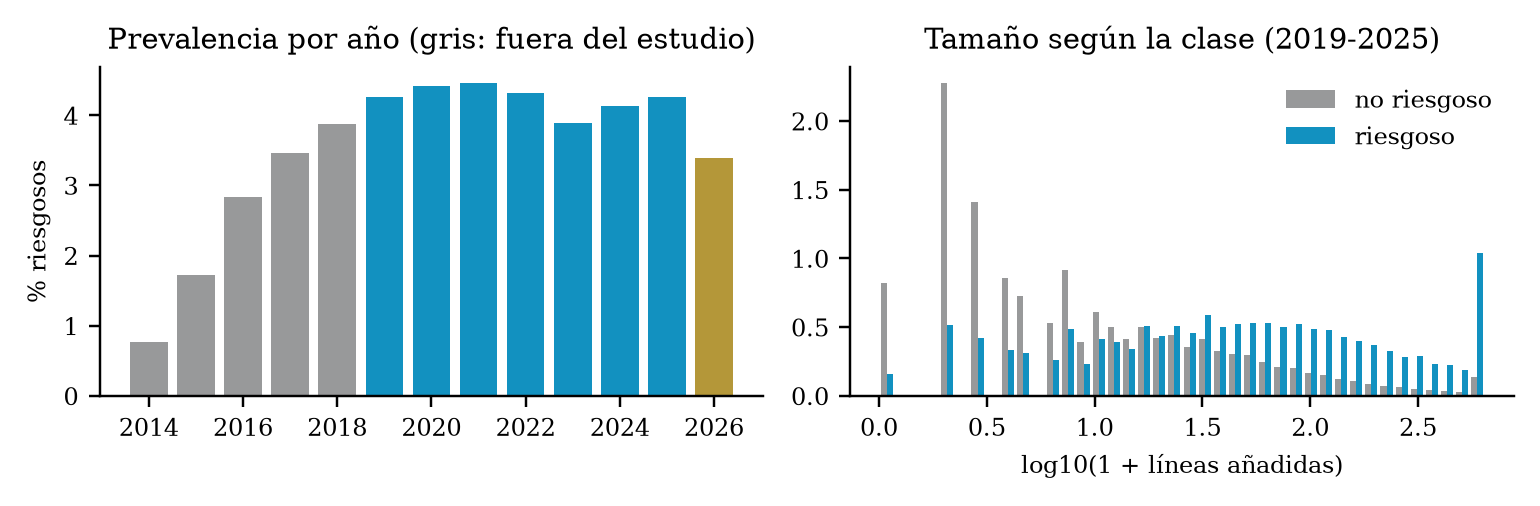
\includegraphics[width=\linewidth]{../../resultados/e2/prevalencia_y_tamano.png}\\[4pt]
      {\fontsize{8pt}{9.5pt}\selectfont Antes de 2019 la prevalencia sube por la adopción de \texttt{Fixes:}, así que se entrena desde 2019. El tamaño es la señal dominante: la prevalencia va de \cifPrevQunoAdd{} a \cifPrevQcincoAdd{} entre quintiles. Ya hay deriva antes de 2026: \texttt{Reviewed-by} por commit pasa de \cifReviewedIni{} a \cifReviewedFin{}.}
    \end{column}
  \end{columns}
\end{frame}

%-------------------------------------------------------------------
\begin{frame}{Modelo y protocolo}{Sistema difuso genético tipo Pittsburgh}
  \begin{columns}[T,onlytextwidth]
    \begin{column}{0.50\textwidth}
      \begin{tikzpicture}[x=2.4cm,y=1.1cm,font=\scriptsize]
        \draw[UDSable,->] (0,0) -- (1.08,0) node[right] {$z$};
        \draw[UDSable,->] (0,0) -- (0,1.15) node[above] {$\mu$};
        \draw[UDBlue,thick] (0,1) -- (0.25,1) -- (0.55,0);
        \draw[UDGold,thick] (0.25,0) -- (0.55,1) -- (0.8,0);
        \draw[UDGreen,thick] (0.55,0) -- (0.8,1) -- (1,1);
        \foreach \x/\l in {0.25/a,0.55/b,0.8/c} \draw (\x,0) -- (\x,-0.05) node[below] {$\l$};
        \node[UDBlue] at (0.12,1.12) {bajo}; \node[UDGold] at (0.55,1.12) {medio}; \node[UDGreen] at (0.92,1.12) {alto};
      \end{tikzpicture}\\[3pt]
      {\fontsize{8pt}{9.5pt}\selectfont
      Cuantiles $\to$ 3 términos de Ruspini $\to$ reglas de $\le$3 antecedentes (producto, O probabilístico).\\
      El AG ajusta vértices y reglas; aptitud = AUC-PR $-\ \lambda\cdot$antecedentes.\\
      \textbf{Variante sin evolución:} la solución voraz que siembra el AG.}
    \end{column}
    \begin{column}{0.46\textwidth}
      {\fontsize{8pt}{9.5pt}\selectfont
      \textbf{Referencias:} clase mayoritaria, regresión logística, \emph{gradient boosting}.\\[4pt]
      \textbf{Partición temporal:} validación creciente 2023, 2024, 2025 con hueco de 90 días; prueba ene--jul 2026, evaluada \textbf{una vez}, con huella SHA-256.\\[4pt]
      \textbf{Métricas:} AUC-PR (principal), MCC, AUC-ROC, IC 95\,\% \emph{bootstrap}, McNemar, Friedman--Nemenyi.\\[4pt]
      \textbf{Entrenamiento:} búsqueda aleatoria (14 configuraciones), sensibilidad 3$\times$3, 5 semillas, configuración congelada.}
    \end{column}
  \end{columns}
  \note{4 min entre esta y la anterior.}
\end{frame}

%-------------------------------------------------------------------
\begin{frame}{Experimentación en validación}{La evolución mejora y simplifica}
  \begin{columns}[T,onlytextwidth]
    \begin{column}{0.48\textwidth}
      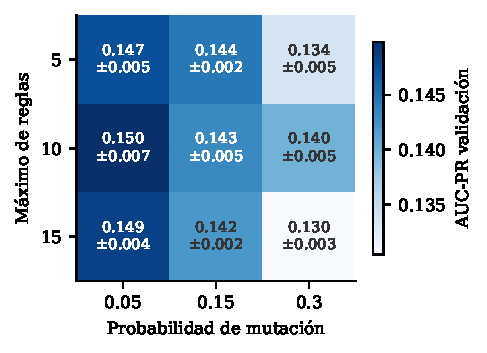
\includegraphics[width=0.92\linewidth]{../../resultados/figuras/sensibilidad.pdf}\\
      {\fontsize{7.5pt}{8.5pt}\selectfont Mutación baja gana (\cifSensMutBaja{} frente a \cifSensMutAlta{}); el máximo de reglas casi no importa.}
    \end{column}
    \begin{column}{0.48\textwidth}
      {\fontsize{8.5pt}{10pt}\selectfont
      \begin{tabular}{@{}lr@{}}
      \toprule
      Modelo (AUC-PR validación) & \\
      \midrule
      \emph{Gradient boosting} & \cifValGB\\
      \textbf{Difuso-evolutivo} (5 semillas) & \textbf{\cifValFE}\\
      Regresión logística & \cifValLogistica\\
      Sin evolución & \cifValVariante\\
      Clase mayoritaria & \cifValMayoritaria\\
      \bottomrule
      \end{tabular}}\\[8pt]
      \UDCard{UDLightGray}{UDBlue!60}{\cardtitle{UDBlue}{Hallazgo}{\fontsize{8.5pt}{10pt}\selectfont
      Sin evolución: \cifReglasVariante{} reglas, \cifAntVariante{} antecedentes.\\ Con evolución: \textbf{\cifReglasMin--\cifReglasMax{} reglas} y más AUC-PR.}}
    \end{column}
  \end{columns}
\end{frame}

%-------------------------------------------------------------------
\begin{frame}{Resultados en 2026}{\cifNPrueba{} commits, prevalencia \cifPrevPrueba{}, evaluación única}
  \begin{columns}[T,onlytextwidth]
    \begin{column}{0.52\textwidth}
      {\fontsize{8.5pt}{10pt}\selectfont
      \begin{tabular}{@{}lcc@{}}
      \toprule
      Modelo & AUC-PR & Caída\\
      \midrule
      \emph{Gradient boosting} & \cifTestGB & \cifCaidaGB\\
      Regresión logística & \cifTestLR & \cifCaidaLR\\
      \textbf{Difuso-evolutivo} & \textbf{\cifTestFE} & \cifCaidaFE\\
      Sin evolución & \cifTestVar & \cifCaidaVar\\
      Clase mayoritaria & \cifTestMay & --\\
      \bottomrule
      \end{tabular}}\\[8pt]
      {\fontsize{8.5pt}{10pt}\selectfont
      \textbf{C1 se cumple:} \cifCuno{} (meta 90\,\%).\\
      \textbf{C2 no se cumple:} cae más que el GB.\\
      \textbf{C3 parcial:} IC \cifTestFEic{} excluye la prevalencia, pero McNemar favorece a las referencias.\\
      Friedman $p=\cifFriedmanP$; Nemenyi CD = \cifNemenyiCD.}
    \end{column}
    \begin{column}{0.44\textwidth}
      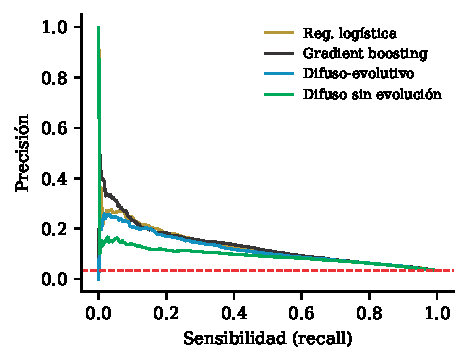
\includegraphics[width=\linewidth]{../../resultados/figuras/curvas_pr.pdf}
    \end{column}
  \end{columns}
  \note{4 min entre esta y la siguiente: resultado negativo, reportado tal cual.}
\end{frame}

%-------------------------------------------------------------------
\begin{frame}{Qué aprendió y dónde falla}{Interpretabilidad y umbral}
  \begin{columns}[T,onlytextwidth]
    \begin{column}{0.54\textwidth}
      \UDCard{white}{UDBorder}{\cardtitle{UDBlue}{Las \cifNReglasRef{} reglas (semilla de referencia)}{\fontsize{7.6pt}{9.2pt}\selectfont
      R1 (0,62) líneas añadidas alto ($\ge$16)\\
      R2 (0,29) líneas añadidas alto Y archivos alto ($\ge$2)\\
      R3 (0,21) un subsistema Y no borra líneas\\
      R4 (0,13) $\ge$2 subsistemas Y borra 1--4 líneas\\
      R5 (0,12) $\ge$2 subsistemas}}
      \vspace{0.12cm}
      {\fontsize{8pt}{9.5pt}\selectfont \cifParamFE{} parámetros frente a \cifParamGBprueba{} del \emph{gradient boosting}.}
    \end{column}
    \begin{column}{0.42\textwidth}
      {\fontsize{8.3pt}{10pt}\selectfont
      \textbf{El umbral no se transfiere:} con pocas reglas el puntaje es escalonado; el corte de 2025 marca entre \cifFEMarcMin{} y \cifFEMarcMax{} de 2026 según la semilla.\\[5pt]
      \textbf{Errores:} no marca commits pequeños (sensibilidad 0 en los tres quintiles inferiores) y rinde menos en correcciones (\cifErrFixAp{} frente a \cifErrNoFixAp).\\[5pt]
      \textbf{\texttt{Assisted-by}:} todos rinden peor (difuso \cifAssistedFE{}, GB \cifAssistedGB).}
    \end{column}
  \end{columns}
\end{frame}

%-------------------------------------------------------------------
\begin{frame}{Iteración 2 y limitaciones}{CRISP-ML(Q): volver al modelado, con reglas fijadas antes}
  \begin{columns}[T,onlytextwidth]
    \begin{column}{0.48\textwidth}
      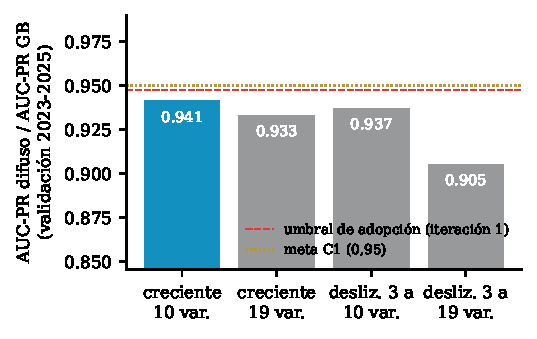
\includegraphics[width=0.95\linewidth]{../../resultados/figuras/iteracion2_candidatos.pdf}\\
      {\fontsize{7.8pt}{9pt}\selectfont Ventana deslizante de 3 años y 19 variables: ninguna supera a la iteración 1 en validación. \textbf{No se adoptó y la prueba no se volvió a usar.}}
    \end{column}
    \begin{column}{0.48\textwidth}
      {\fontsize{8.3pt}{10pt}\selectfont
      \begin{itemize}
        \item La prueba se miró con modelos simples en la factibilidad; se declara.
        \item \texttt{Fixes:} acierta el $\sim$81\,\%; la censura ignora errores tardíos.
        \item \texttt{Assisted-by} es una cota inferior.
        \item Un solo proyecto; la búsqueda quedó en el borde del espacio.
        \item McNemar con umbral fijo castiga a quien marca más.
      \end{itemize}}
    \end{column}
  \end{columns}
\end{frame}

%-------------------------------------------------------------------
\begin{frame}{Conclusiones}{}
  \begin{columns}[T,onlytextwidth]
    \begin{column}{0.31\textwidth}
      \UDCard{white}{UDBorder}{\cardtitle{UDBlue}{No alcanzó la meta}{\fontsize{8.5pt}{10pt}\selectfont \cifCuno{} del GB y más caída en 2026 (\cifCaidaFE{} frente a \cifCaidaGB). Se reporta tal cual.}}
    \end{column}
    \begin{column}{0.31\textwidth}
      \UDCard{white}{UDBorder}{\cardtitle{UDBlue}{Pero es útil y legible}{\fontsize{8.5pt}{10pt}\selectfont 3,5$\times$ la prevalencia con 3--6 reglas; la evolución aporta \cifAporteEvolPrueba{} y simplifica.}}
    \end{column}
    \begin{column}{0.31\textwidth}
      \UDCard{white}{UDBorder}{\cardtitle{UDBlue}{Siguiente paso}{\fontsize{8.5pt}{10pt}\selectfont Recalibrar el umbral con datos recientes y premiar la estabilidad temporal en la aptitud.}}
    \end{column}
  \end{columns}
  \vspace{0.4cm}
  {\centering\fontsize{9pt}{11pt}\selectfont La interpretabilidad cuesta $\sim$9 puntos de AUC-PR y no dio robustez frente a la deriva de 2026.\par}
  \note{2 min.}
\end{frame}

\UDcierre{Juan Felipe Rodríguez Galindo}
         {Maestría en Ciencias de la Información\\y las Comunicaciones}
         {Inteligencia Computacional}

\end{document}
